\chapter{Proof of theorem}\label{app:Proof of theorem}
\lipsum[1]
\begin{figure}[thbp]
    \centering
    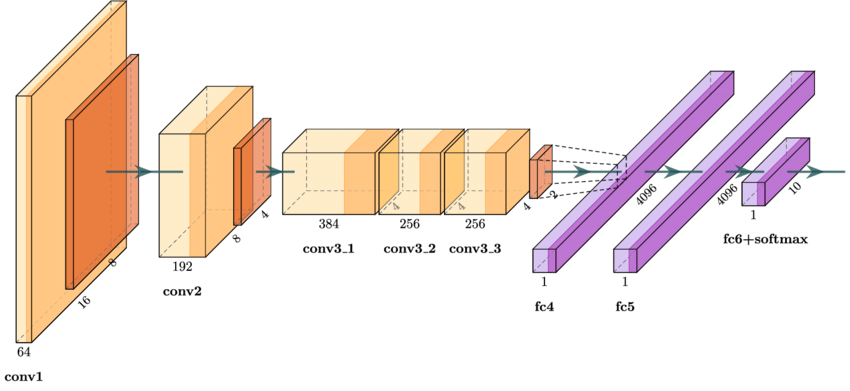
\includegraphics[width=\textwidth]{img/appendixA/alexnet.png}
    \caption{AlexNet architecture.}\label{fig:alexnet}
\end{figure}
\lipsum[1]
\begin{align}
     \vec{\nabla} \cdot \vec{E} \quad &=\quad\frac{\rho}{\epsilon_0} &&\text{Gauss's Law} \\      
    \vec{\nabla} \cdot \vec{B} \quad &=\quad 0 &&\text{Gauss's Law for Magnetism}\\
    \vec{\nabla} \times \vec{E} \quad &=\hspace{10pt}-\frac{\partial{\vec{B}}}{\partial{t}} &&\text{Faraday's Law of Induction} \\ 
    \vec{\nabla} \times \vec{B} \quad &=\quad \mu_0\left( \epsilon_0\frac{\partial{\vec{E}}}{\partial{t}}+\vec{J}\right) &&\text{Ampere's Circuital Law}
\end{align}

We can find more information in~\cite{li2018deep}.

